\section{Methods for concept drift adaptation}
% ------------------------------------------------------------------------------
\begin{frame}
\frametitle{Agenda}
\tableofcontents[currentsection]
\end{frame}
% ------------------------------------------------------------------------------


% --------------------------------------------------------------------------------------------------------------
\begin{frame}
\frametitle{Methods for concept drift adaptation}

\begin{figure}[H]
	\centering
	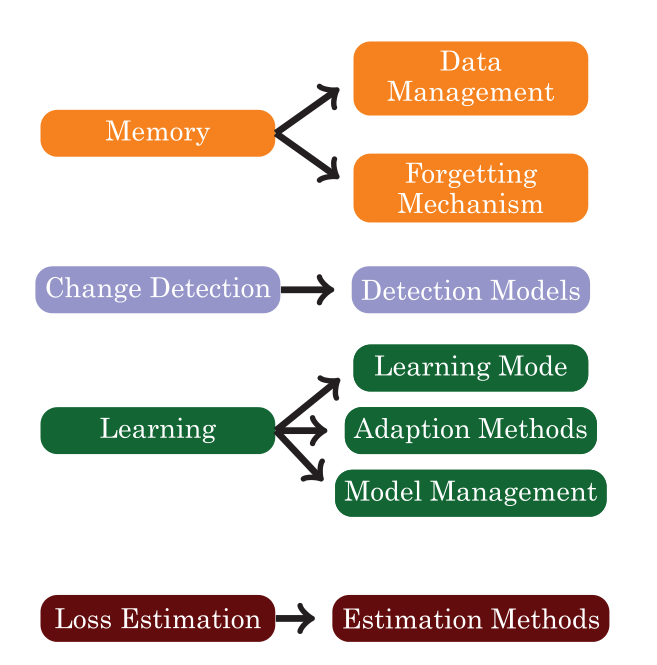
\includegraphics[scale=0.25]{mfcda/fourmodules}
\end{figure}

\end{frame}


\begin{frame}
\frametitle{Methods for concept drift adaptation}

\begin{figure}[H]
	\centering
	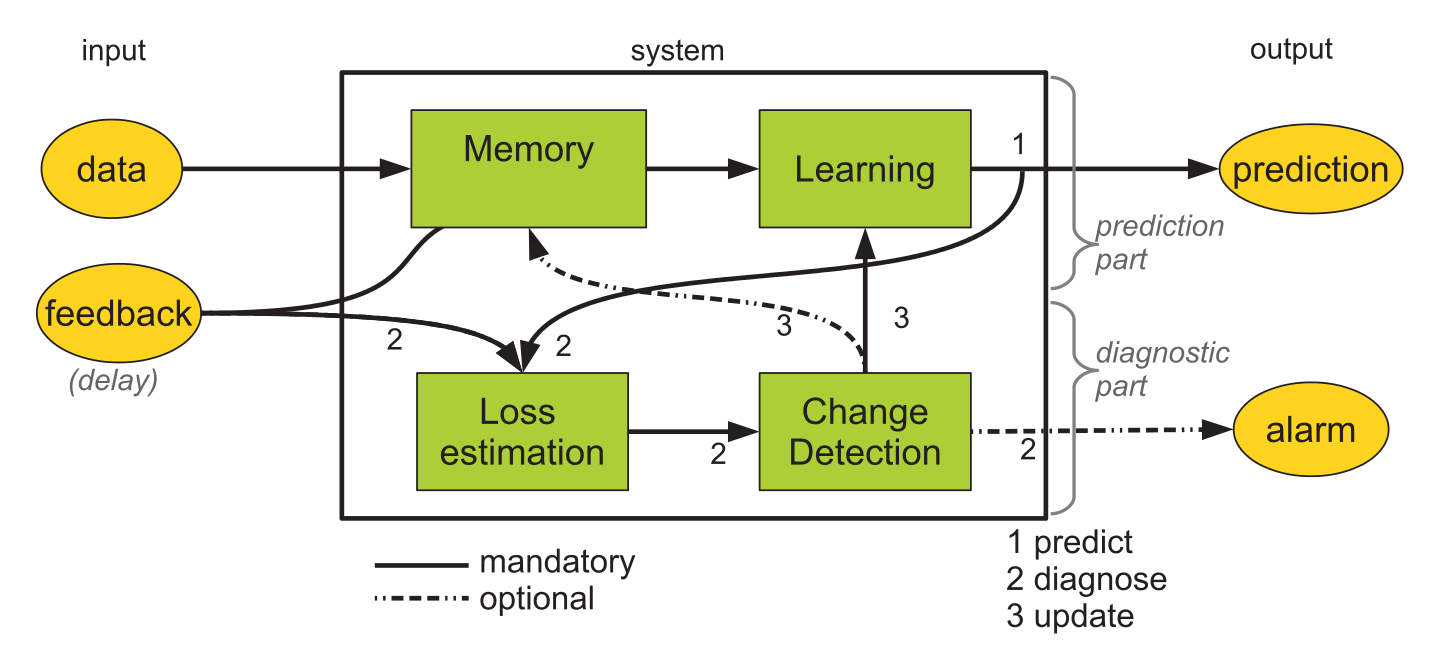
\includegraphics[width=\textwidth]{modelala}
\end{figure}

\end{frame}
% --------------------------------------------------------------------------------------------------------------

\subsection{Memory}

% ------------------------------------------------------------------------------
\begin{frame}
\frametitle{Agenda}
\tableofcontents[currentsubsection]
\end{frame}
% ------------------------------------------------------------------------------

% --------------------------------------------------------------------------------------------------------------
\begin{frame}
\frametitle{Memory in concept drift Adaptation}

\begin{figure}[H]
	\centering
	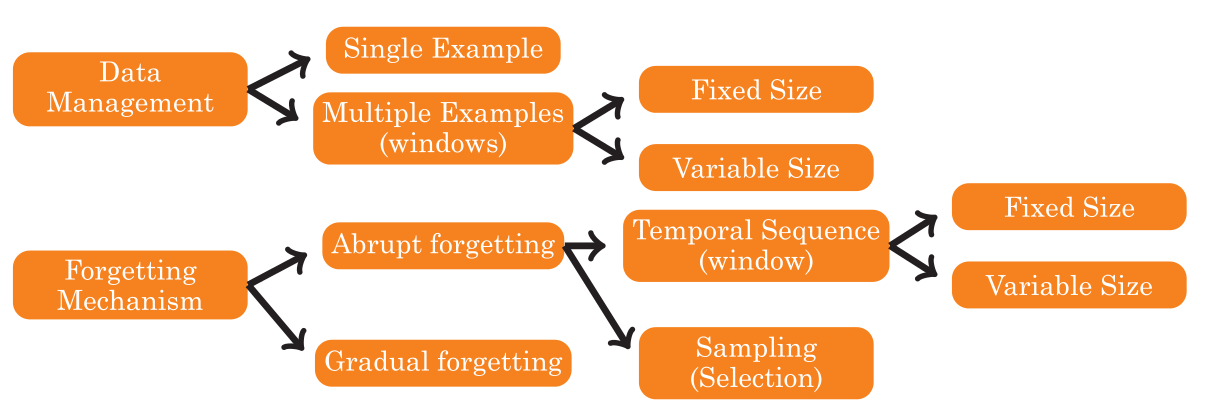
\includegraphics[width=\textwidth]{mfcda/memory}
\end{figure}

\end{frame}
% --------------------------------------------------------------------------------------------------------------


\begin{frame}
\frametitle{Data Management}

\begin{figure}[H]
	\centering
	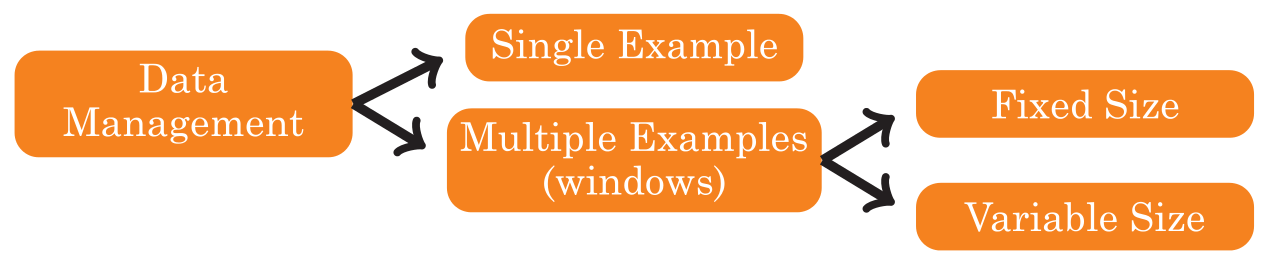
\includegraphics[width=0.8\textwidth]{mfcda/datamanagement}
\end{figure}


Often is assumed that the most recent data is the most informative.
\begin{itemize}
	\item \textbf{Single example:} almost no memory needed, more error prone.\\
	Sometimes necessary because of speed and memory constraints (e.g. in online learning and streaming)
	\item \textbf{ Multiple examples:} a set of recent examples:
	\begin{itemize}
		\item \textit{Fixed size:} often used as baseline
		\item \textit{Variable size:} depending on idication of a change detector
	\end{itemize}
\end{itemize}

\end{frame}



\begin{frame}
\frametitle{Forgetting mechanism}

\begin{figure}[H]
	\centering
	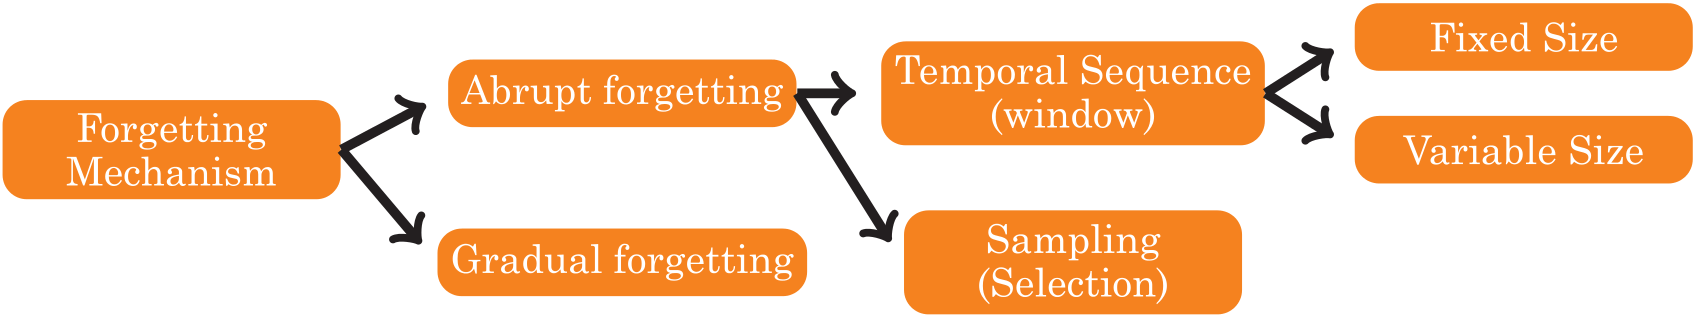
\includegraphics[width=0.9\textwidth]{mfcda/forgetting}
\end{figure}

\begin{itemize}
	\item \textbf{Abrupt forgetting:} a window considered for learning.
	\item \textbf{Gradual forgetting:} examples are not really discarded, they are associated with weights.
\end{itemize}


\end{frame}






\subsection{Change Detection}

% ------------------------------------------------------------------------------
\begin{frame}
\frametitle{Agenda}
\tableofcontents[currentsubsection]
\end{frame}
% ------------------------------------------------------------------------------

\begin{frame}
\frametitle{Change detection}

\begin{figure}[H]
	\centering
	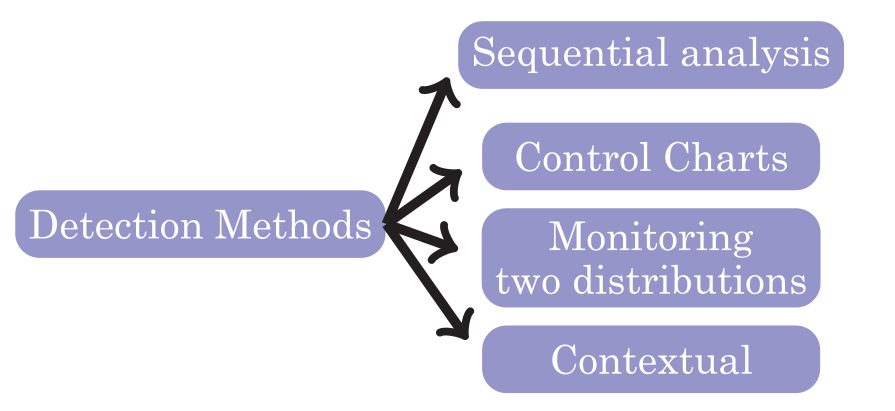
\includegraphics[width=0.55\textwidth]{mfcda/detection}
\end{figure}

\begin{itemize}
	\item \textbf{Sequential analysis:} detectors use sequential analysis e.g. \textit{Sequential Probability Ratio Test}
	\item \textbf{Statistical Process Control (SPC):} standard statistical techniques to predict change.
	\item \textbf{Monitoring distributions on two different time windows:}
	\only<2>{
	\begin{itemize}
		\item one fixed reference window (summarizes the past information)
		\item one sliding window over the the most recent examples
		\item distributions are compared using statistical tests
	\end{itemize}
		}
	\only<3>{
	\item \textbf{Contextual approaches:} a learning techinique that identifies intervals with stable hidden context
	}	 
\end{itemize}

\end{frame}



\subsection{Learning}

% ------------------------------------------------------------------------------
\begin{frame}
\frametitle{Agenda}
\tableofcontents[currentsubsection]
\end{frame}
% ------------------------------------------------------------------------------

\begin{frame}
\frametitle{Learning}

\begin{figure}[H]
	\centering
	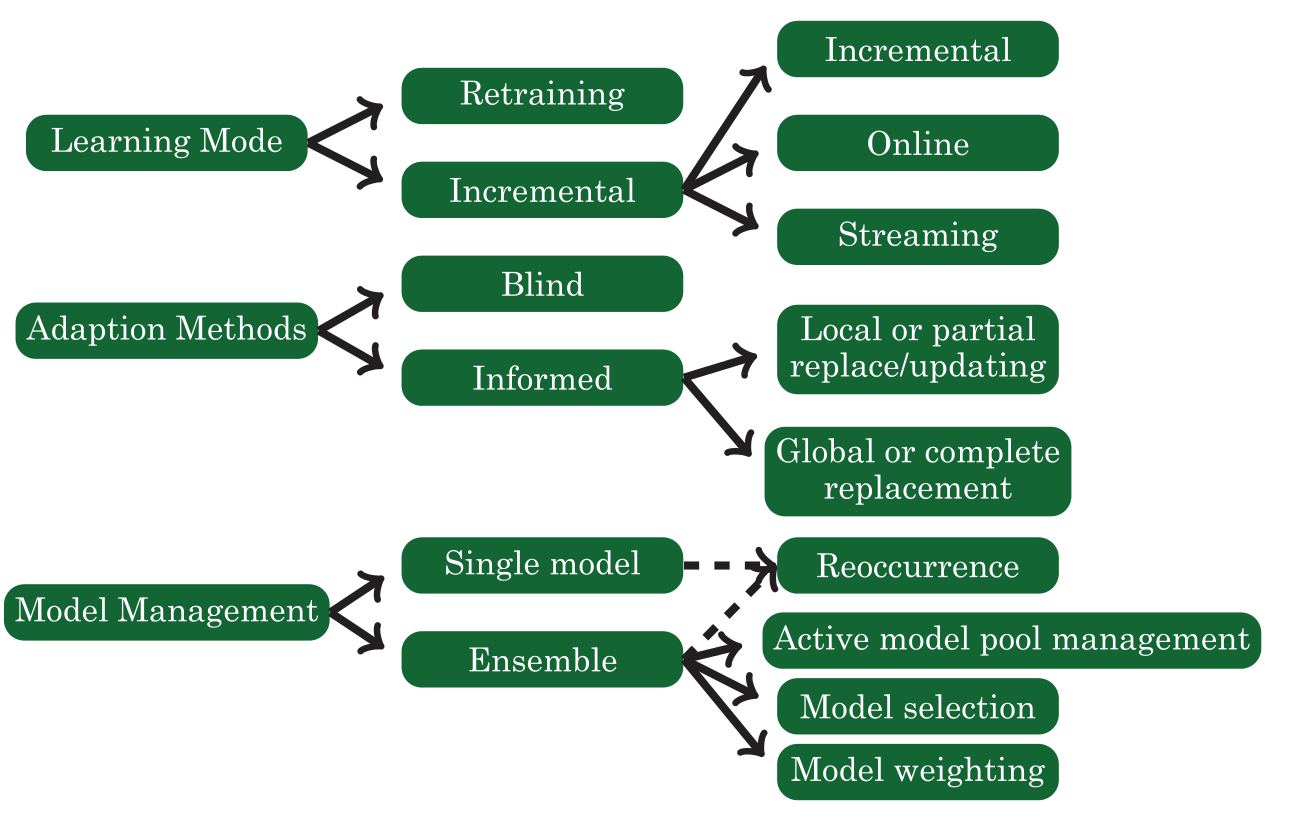
\includegraphics[width=\textwidth]{mfcda/learning}
\end{figure}



\end{frame}


\begin{frame}
\frametitle{Learning mode}

\begin{figure}[H]
	\centering
	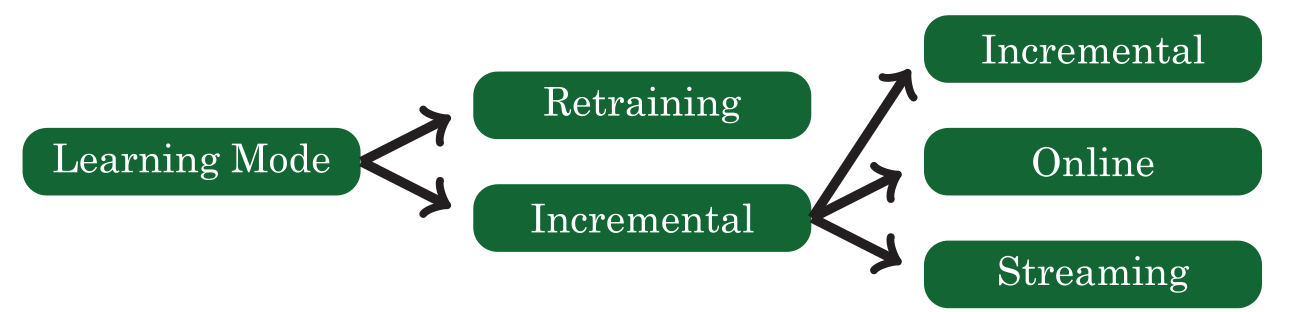
\includegraphics[width=0.8\textwidth]{mfcda/mode}
\end{figure}
If new labeled examples are available the model might be updated:
\begin{itemize}
	\item \textbf{Retraining:} start from scratch, using bufferd data.
	\only<2>{
	\item \textbf{Incremental:} update the model using most recent data:
		\begin{itemize}
			\item \textbf{Incremental:} modify and update statistics in the model upon arrival from new examples (can still have acces to old values)
			\item \textbf{Online:} update the current model with most recent example $\rightarrow$ errorprone if last example is misclassified
			\item \textbf{Streaming:} are online algorithms for a high-speed continious flow of data. Limited memory and normally only one pass over the data.
		\end{itemize}
		}
\end{itemize}

\end{frame}


\begin{frame}
\frametitle{Adaption Methods}
\begin{figure}[H]
	\centering
	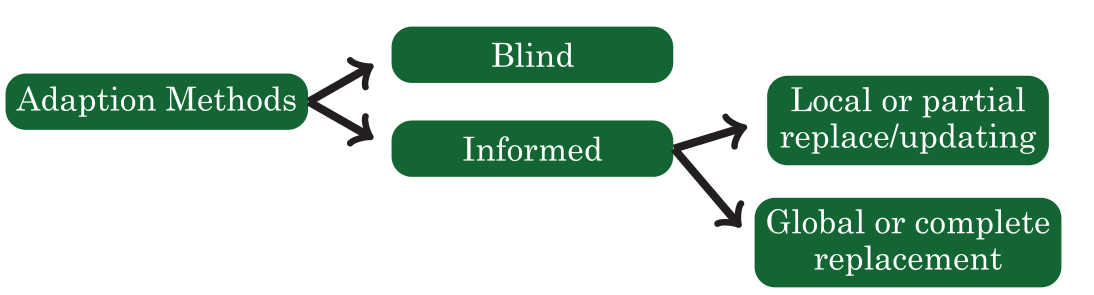
\includegraphics[width=0.8\textwidth]{mfcda/adaption}
\end{figure}

\begin{itemize}
	\item Manage the adaptation of the predictive model
	\begin{itemize}
		\item \textbf{Blind:} without explicit detection of changes. (fixed-size sliding windows)
		\item \textbf{Informed:} action depend triggers:
		\begin{itemize}
			\item \textit{Global Replacement:} the model is rebuild (linear regression, naive Bayes...)
			\item \textit{Local Replacement:} if the model is modular (e.g. a decision tree) only a part (e.g. a subtree) is replaced
			
		\end{itemize}
	\end{itemize}
\end{itemize}


\end{frame}

\begin{frame}
\frametitle{Adaption Methods}
\begin{figure}[H]
	\centering
	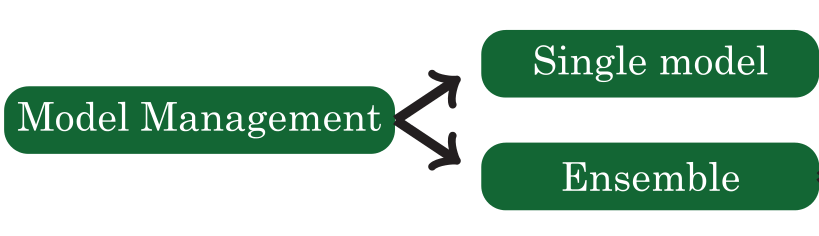
\includegraphics[width=0.65\textwidth]{mfcda/modelmanagement}
\end{figure}

\begin{itemize}
	\item \textbf{Single model:} only a single model is used
	\item \textbf{Ensemble:} multiple models are used together and do voting
\end{itemize}


\end{frame}



\subsection{Loss Estimation}

% ------------------------------------------------------------------------------
\begin{frame}
\frametitle{Agenda}
\tableofcontents[currentsubsection]
\end{frame}
% ------------------------------------------------------------------------------


% --------------------------------------------------------------------------------------------------------------
\begin{frame}
\frametitle{Loss estimation in concept drift Adaptation}

\begin{figure}[H]
	\centering
	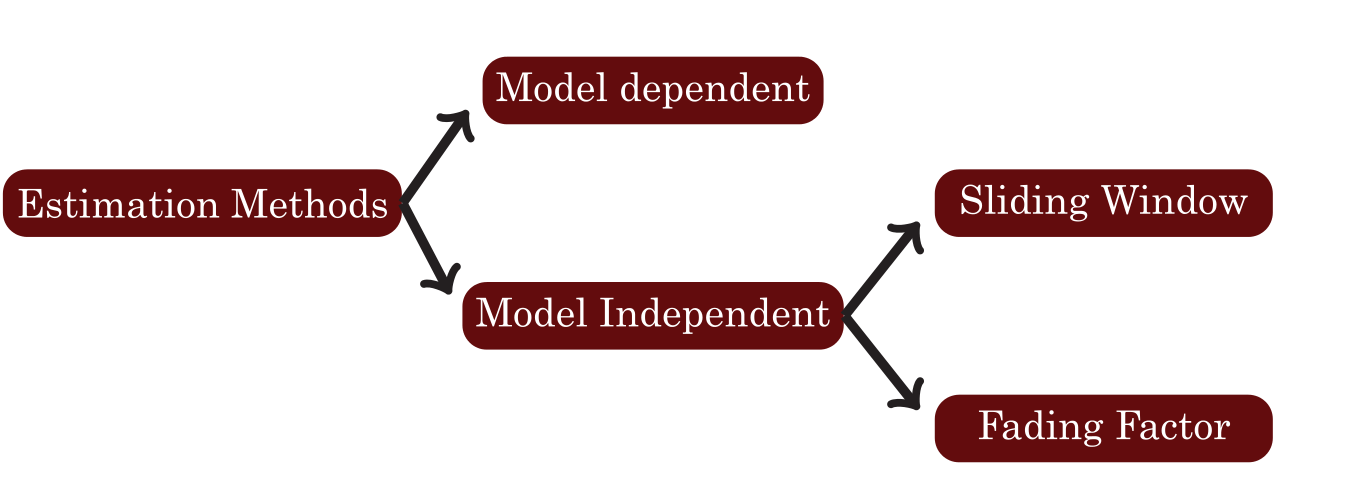
\includegraphics[scale=0.2]{mfcda/loss}
\end{figure}
\only<2>{
\begin{itemize}

\item \textbf{Model Dependent}
	\begin{itemize}
	\item Estimator needs to learn from the current model
	\item e.g. Klinkenbeg and Joachims \cite{klinkenberg} use it in SVM
	\end{itemize}

\end{itemize}
}

\only<3>{
\begin{itemize}

\item \textbf{Model Independent}
	\begin{itemize}
	\item Can be applied immediately
	\item \textbf{Sliding Window:} one small (quick) and one large (slower) together
	\item \textbf{Fading Factor:} a small FF detects change earlier
	\end{itemize}
\end{itemize}
}

\end{frame}




% --------------------------------------------------------------------------------------------------------------
